% Created 2016-04-17 Son 19:46
\documentclass[11pt, a4paper]{article}
\usepackage[utf8]{inputenc}
\usepackage[T1]{fontenc}
\usepackage{fixltx2e}
\usepackage{graphicx}
\usepackage{longtable}
\usepackage{float}
\usepackage{wrapfig}
\usepackage{soul}
\usepackage{textcomp}
\usepackage{marvosym}
\usepackage{wasysym}
\usepackage{latexsym}
\usepackage{amssymb}
\usepackage{hyperref}
\tolerance=1000
\usepackage{minted}
\usepackage[utf8]{inputenc}
\usepackage[english]{babel}
\usepackage{graphicx}
\usepackage[left=2.35cm, right=3.35cm, top=3.35cm, bottom=3.0cm]{geometry}
\usepackage{titling}
\providecommand{\alert}[1]{\textbf{#1}}

\title{Statistical methods for bioinformatics \linebreak Model selection and regularization}
\author{Cedric Lood}
\date{\today}
\hypersetup{
  pdfkeywords={},
  pdfsubject={},
  pdfcreator={Emacs Org-mode version 7.9.3f}}

\begin{document}

\maketitle


\graphicspath{ {figures/} }
\setlength{\droptitle}{-5em} 
\setlength{\parindent}{0cm}

\section{Conceptual exercises}
\label{sec-1}
\subsection{Question 5}
\label{sec-1-1}
\subsubsection{part a}
\label{sec-1-1-1}

We want to minimize the ridge regression defined by $RSS + \lambda \sum\limits_{i=1}^p \hat{\beta}_i^2$

\begin{itemize}
\item $min\Big[\sum\limits_{i=1}^n {(y_i - \hat{\beta}_0 - \sum\limits_{j=1}^p {\hat{\beta}_jx_j} )^2} + \lambda \sum\limits_{i=1}^p \hat{\beta}_i^2\Big]$
\item we have as constraints that $\hat{\beta}_0 = 0, p=2$, hence we can
  reformulate the optimisation as $min\Big[\sum\limits_{i=1}^n {(y_i - \sum\limits_{j=1}^2 {\hat{\beta}_jx_j} )^2} + \lambda \sum\limits_{i=1}^2 \hat{\beta}_i^2\Big]$
\item which can be expanded into $min\Big[ (y_1 - \hat{\beta}_1x_{11} - \hat{\beta}_2x_{12})^2 + (y_2 - \hat{\beta}_1x_{21} - \hat{\beta}_2x_{22})^2 + \lambda (\hat{\beta}_1^2 + \hat{\beta}_2^2)\Big]$
\end{itemize}
\subsubsection{part b}
\label{sec-1-1-2}

For this, we can simply take the derivatives of the ridge regression
with respect to $\hat{\beta}_1$ and $\hat{\beta}_2$.
\subsubsection{part c}
\label{sec-1-1-3}

Very similar to part a, the only difference between the lasso method
and the ridge regression lies with the norm taken of the
parameters. Lasso used a first-order norm (L1):

$min\Big[ (y_1 - \hat{\beta}_1x_{11} - \hat{\beta}_2x_{12})^2 + (y_2 - \hat{\beta}_1x_{21} - \hat{\beta}_2x_{22})^2 + \lambda (|\hat{\beta}_1| + |\hat{\beta}_2|)\Big]$
\section{Applied exercises}
\label{sec-2}
\subsection{Question 8}
\label{sec-2-1}


\begin{minted}[]{R}
library(ggplot2)

## part a: simulated dataset creation
set.seed(1)
x <- rnorm(100)
noise <- rnorm(100)

## part b: response vector with given model y = 1x^3 - 2x^2 + 3x + 5
y <- x^3 - 2*x^2 + 3*x + 5
qplot(x,y)
ggsave("fun.pdf")
\end{minted}

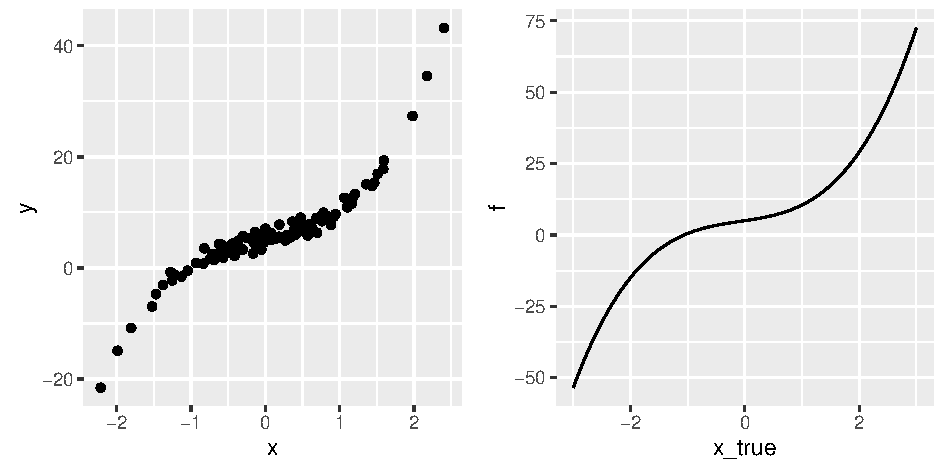
\includegraphics[scale=0.5]{fun.pdf}
\subsection{Question 10}
\label{sec-2-2}

\end{document}
